\chapter{Introduction}
\section{Background}
The disaster is divided to two types. The first one is disaster caused by human behavior such as fires, accidents, terrorism and murder. The other one is disaster occurred because of factors of nature itself such as floods, earthquakes, tsunamis and volcanic eruptions. The threatening of disaster can happen anytime or anywhere, and humans  can not avoid the risk of disaster. The most likely thing to do is to reduce the impact/risk and prepare the community in facing the disaster. there are many ways was developed and researched to prevent or reduce disaster impact, One of them is using disaster risk management (Disaster Management).\par
In recent years, Indonesia is very close to the many disasters. In line with it, Indonesia also has a serious problem in disaster prevention. There are many problems caused Indonesia become disaster area easily. Indonesia has many rivers, many active volcanoes, high rainfall and social economical habit. In the city, likes Jakarta and Bandung, Indonesia has flood as main problem and in rural area such as village, Indonesia has drought, avalanche and volcanoes eruption.  National Agency for Disaster Management (BNPB) states that between 1996 to 2014 Indonesia has three main problem disaster, that are flood, tsunami and drought\cite{DataBNPB}. The United Nations International Strategy for Disaster Reduction (UN-ISDR) ranks Indonesia at sixth biggest, with a loss of US \$27.84 billions in economical damage in 1991 to 2005. The data is not including the giant Tsunami disaster in 2004 and in few years later, the losses number can increase more and more.\par

\begin{figure}[h!]
\centering
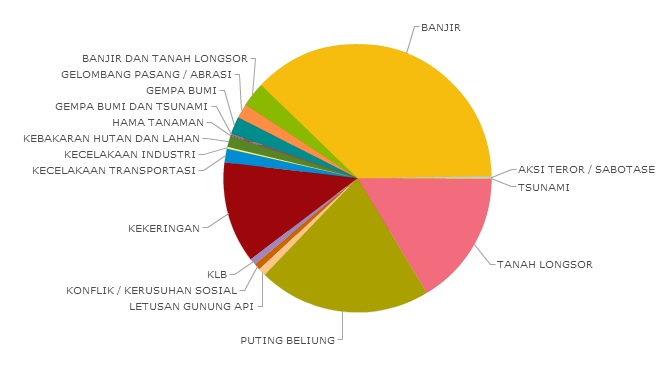
\includegraphics[scale=0.7]{StatistikBencana.png}
\caption{\small Comparison of numbers of disasters between 1815 to 2014\cite{DataBNPB}}
\label{fig:StatBen}
\end{figure}

In January 2005\cite{HFAConference}, Indonesia Government uses a 10-year plan to make the world safer from natural hazard. The framework was named by Hyogo for Action (HFA) Framework. Substantively, The framework is not the first introduced to the world, because before using HFA, some global communities used Yokohama Strategy and Plan for Safer World as a unique opportunity to promote systematic and strategic approaches at the national level to address vulnerability and reduce the risk to natural hazards. In his improvisation, HFA framework has fives important and priority actions as a global blueprint to reduce disaster losses by 2015 in lives, economic and environmentally assets of communities and country.\par
Therefore, this research purposed an intelligent model of Disaster Management based on service system. In line with Service System Engineering (SSE) is becoming the huge development research in providing the services, the system that will be created has many opportunity to achieve HFA Framework purposes. SSE services many sector in communities live, where economy is the main sectors. In disaster management content, SSE will service environmental assets of communities as main sector and country as the sub sectors. Some researchers are utilizing a socio-economic and technological perspective to investigate end-user (customer) interactions with government organization or agency by developing formal methodologies for value co-creation and productivity improvements\cite{Lopes2013}. Technological perspective can wipe off some mistake of communities habit in disaster mitigation, provide the best way of getting disaster information, economize the cost expended and help disaster management agency providing services better.\par

\section{Statements of Problems}
\label{sec:StateOfProblem}
According to national progress report on the implementation of HFA (2011-2013)\cite{Framework2013}, there are many problem in disaster management (DM) implementation. One of them is the lack of synchronization between DM-related and non DM-regulation, such as those related to investment and economic development. The problems come from disharmony in regulatory of framework between any levels in government. And it can postpone the  more effective integration of disaster risk considerations into sustainable development policies, planning and programming at all levels, with a special emphasis on disaster prevention, mitigation, preparedness and vulnerability reduction\par
\begin{comment}
	masalah yangmuncul:
	1. Rendahnya proses sinkronisasi DM-related and non DM-Regulation ... apa itu DM related dan regulation,,, contohnya dalam investment dan ekonomi
	emphasis = penekanan

\end{comment}

Another problem of disaster mitigation process came from the society or community. A variety of disasters in Indonesia almost always showing  the same attitude that is a condition of the reactive and unplanned spontaneous as shown by the various stakeholders and communities. Each disaster in Indonesia is almost always colored and followed by a process called as \textit{a milling process}\cite{Kusmiati}, that is a situation where people do not know how to act or respond to disasters because there are no clear guidelines to be or if any such guidelines are not relevant to the conditions faced by society. This part is taking important reason when the amount of victims become huge.\par

Huge areas give more challenges to analyze the proper system that we need. as known as Indonesia ia a archipelago country with five big islands and many small islands, and the problems become harder when the location is a small island and isolated. The helpful effort and victim rescue processes in rare area will be slow and very difficult to be reached in short time. And the last problem is the variety losing of early warning detection devices after being placed in the sea\cite{AlatTsunamiHilang}. Many reason referable to this problem, as one of it is coming from the lacking of disaster education were gave to the communities.\par 

\begin{enumerate}
\setlength{\itemsep}{1.5pt}
\setlength{\parskip}{1.5pt}
\item[1.] Providing disaster management system based on HFA.
\item[2.] Providing the engineering services based on disaster management created.
\item[3.] Combining the Engineering Services and Disaster Management. 
\end{enumerate}\par

\section{Objectives}
The Model of Disaster management provided in this research is a combination between client (customer) and provider of services. The clients in this context are all society or community live in Indonesia and the providers are government and National Disaster Agency. This research will utilize many service engineering concept. Therefore, the objective of this research is how to formulate the disaster management based on appropriate service system engineering and Hyogo for Action Framework concepts.\par

\section{Research Question}
the combining of five important actions in HFA with service system will be the main focus of development disaster management model. The model that will be evolved consist of many possible service system. Possible regulations in providing the management system will be included too but not in specific and complex area.\par

\section{Scope and Limitation}
The scope of this research that will be provided are:
\begin{enumerate}
\setlength{\itemsep}{1.5pt}
\setlength{\parskip}{1.5pt}
\item[1.] Providing Disaster Management Model based on Hyogo for Action Framework
\item[2.] Combining the Disaster Management Provided with Service System Engineering
\item[3.] prototyping the system in mobile application\par
\end{enumerate}

\section{Research Output}
The output this research are a model of disaster management and a prototype of disaster management system. Both of them based on service system engineering. The system will provide a quick responses concept before the disaster attack even when after the attack. This system hopefully will support many cities in Indonesia to solve their problem in providing a good disaster management and give another option in improvisation of theory and application for better disaster management.

\section{Writing Systematic}
The writing systematics in this thesis are consisted of five main part, there are:
\begin{enumerate}
\setlength{\itemsep}{1.5pt}
\setlength{\parskip}{1.5pt}
\item[1.] CHAPTER I Introduction, provides a brief overview of the research background, problem formulation, research objectives, problem definition, research output, as well as systematic discussion.
\item[2.] CHAPTER II Literature, contains the review of the literature, a literature review and reference point-references relating to the cases examined in this study.
\item[3.] CHAPTER III Research Methods, describes the research methodology used as well as the research workflow.
\item[4.] CHAPTER IV Analysis and Design, explains the stages of analysis and design solutions to problems that are based on a theory that has been studied.
\item[5.] CHAPTER V Implementation and Testing, discussed the test scenarios with the aim of reinforcing, proving analysis and design that has been done in Chapter IV as expected
\item[6.] CHAPTER VI Conclusions and Recommendations, the conclusions drawn from the process analysis and modeling systems. As well as the suggestions are expected for the development of research in the future.
\item [7.] REFERENCES, contains a collection of the materials and references used by the author during the making of this thesis statements.
\end{enumerate}
